\section*{ВВЕДЕНИЕ}
\addcontentsline{toc}{section}{ВВЕДЕНИЕ}
\addtocounter{section}{1}
\setcounter{subsection}{0}

Современные объектно ориентированные языки программирования, такие как Java, предоставляют удобные механизмы для написания программ. Java приложения часто работают с большим количеством различных объектов. 
Однако, это может приводить к негативному влиянию на производительность. Огромное число мелких объектов приводит к фрагментации памяти, плохой локальности процессорного кеша, а также к увеличению числа чтений указателей из памяти. Эти факторы неизбежно приводят к ухудшению производительности Java приложения.
\par
В квалификационной работе предлагается способ уменьшения негативного влияния вышеперечисленных недостатков введением в язык Java новой структуры данных, названной flattened array или FlatArray. Эта структура представляет собой последовательность объектов, расположенных в одном линейном участке памяти. 
Для Java программиста flattened массив имеет интерфейс обычного Java класса.
\par
Flattened array может быть применен для реализации многих других структур данных и алгоритмов, зависящих от скорости доступа к памяти. В частности, в данной работе была реализована альтернативная версия хеш-таблицы, которая в некоторых случаях показала лучшую производительность операции поиска.
\par
На рисунке \ref{ref-graph} изображен граф объектов, который может быть частью объектно-ориентированного приложения.
\begin{figure}[h]
	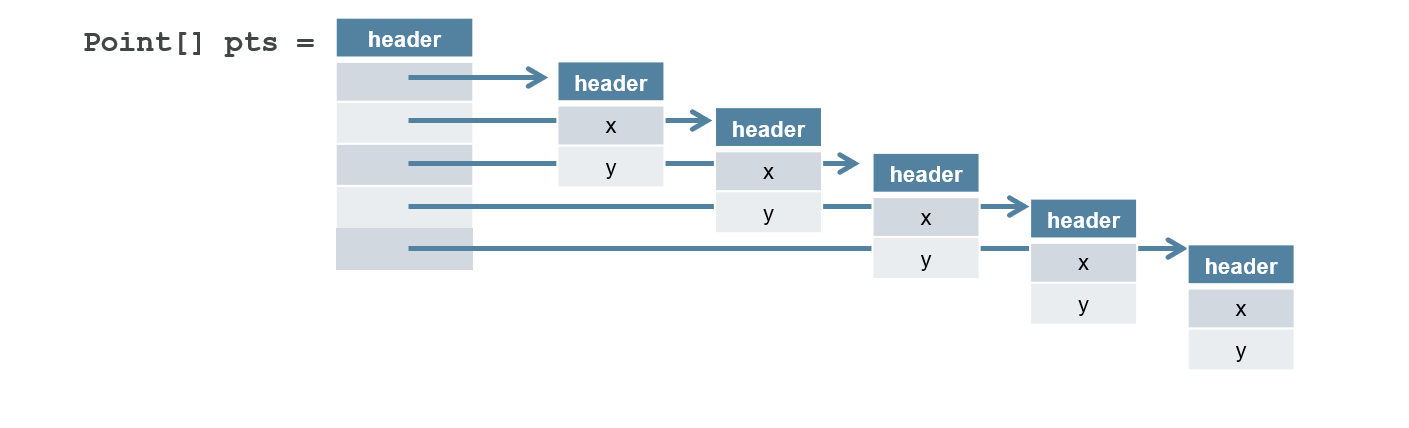
\includegraphics[width=0.95\linewidth]{image/reference.png}
	\caption{Массив объектов класса Point}\label{ref-graph}
\end{figure}
Класс Point содержит в себе два поля x, y типа int. Как описывалось ранее, Java работает с 
такого рода объектами как со ссылками. Потому массив "pts" содержит в себе указатели. В таком случае при доступе к полю "x" элемента i требуется дополнительное разыменования указателя, и только потом поступаемся по поля x.
\begin{lstlisting}
Point value = pts[i].x;
\end{lstlisting}
Однако в реальности мы имеем дополнительные издержки, связанные с исполнением load барьера и проверкой прочитанного значения на null:
\begin{lstlisting}
	Point* tmp = &pts[i];
	Point actual_value = load-barrier(tmp);
	if (actual_value == null) {
		throw new NullPointerException();
	}
\end{lstlisting}
В итоге это приводит к довольно дорогостоящему доступу к элементу массива. Было бы полезно избавиться от дополнительных накладных расходов на доступ к полю. Одним из возможных способов является расположение всего массива в виде линейного участка памяти, как указано на рисунке \ref{values-graph}.

\begin{figure}[h]
	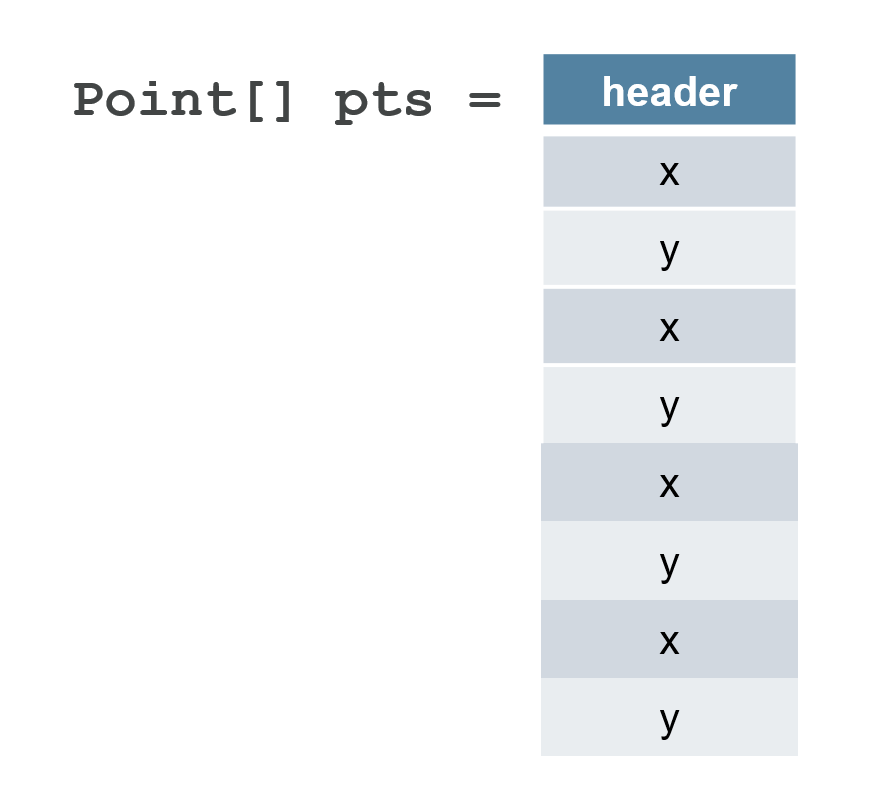
\includegraphics[width=0.65\linewidth]{image/flattened-points.png}
	\caption{Массив значений}\label{values-graph}
\end{figure}
По сравнению с предыдущей раскладкой объектов, у последней есть ряд преимуществ:
\begin{itemize}
	\item Улучшается локальность процессорного кеша. Поскольку объекты находятся рядом, а не разбросаны по всей куче, при чтении одного элемента в линейку кеша могут быть записаны соседние элементы. Это потенциально увеличивает производительность последовательного доступа к элементам массива.
	\item Удаляются load барьер и проверка на null. Адрес конкретного поля i-того элемента могут быть вычислен с помощью простой арифметики. Во многих случаях это обходится дешевле чтения ссылки из памяти. И поскольку виртуальная машина подразумевает, что в таком массиве не бывает указателей, равных null, проверки на null исчезают.
	\item Последовательный доступ к элементам может быть автоматически векторизован компилятором
\end{itemize}
К сожалению, на данный момент JVM и язык Java не поддерживают возможность создания такого рода структуры данных. Разработка такой структуры и поддержка ее в компиляторе и виртуальной машине Java является целью квалификационной работы. Для этой цели необходимо решить следующие задачи: 
\begin{enumerate}
	\item Изучить аналогичные работы
	\item Реализовать данную структуру данных, что подразумевает разработку интерфейса для Java программиста и поддержку на уровне среды исполнения.
	\item Измерить производительность работы со структорой и проанализировать результаты
	\item Изучить применимость новой структуры данных для реализации других структур. Провести тестирование производительности для них.
\end{enumerate}
Данная работа проводилась на базе виртуальной машины Zing. Главными отличиями этой виртуальной машины от OpenJDK является замена С2 компилятором Falcon, базирующемся на LLVM, и применением конкурентного сборщика мусора С4\cite{C4collector}. Ее более подробное описание можно найти в следующей главе.
\clearpage
